% This file was created by matlab2tikz.
%
%The latest updates can be retrieved from
%  http://www.mathworks.com/matlabcentral/fileexchange/22022-matlab2tikz-matlab2tikz
%where you can also make suggestions and rate matlab2tikz.
%
\documentclass[tikz]{standalone}
\usepackage[T1]{fontenc}
\usepackage[utf8]{inputenc}
\usepackage{pgfplots}
\usepackage{grffile}
\pgfplotsset{compat=newest}
\usetikzlibrary{plotmarks}
\usepgfplotslibrary{patchplots}
\usepackage{amsmath}
\usetikzlibrary{decorations.markings}
\usetikzlibrary{shapes,snakes}

\begin{document}

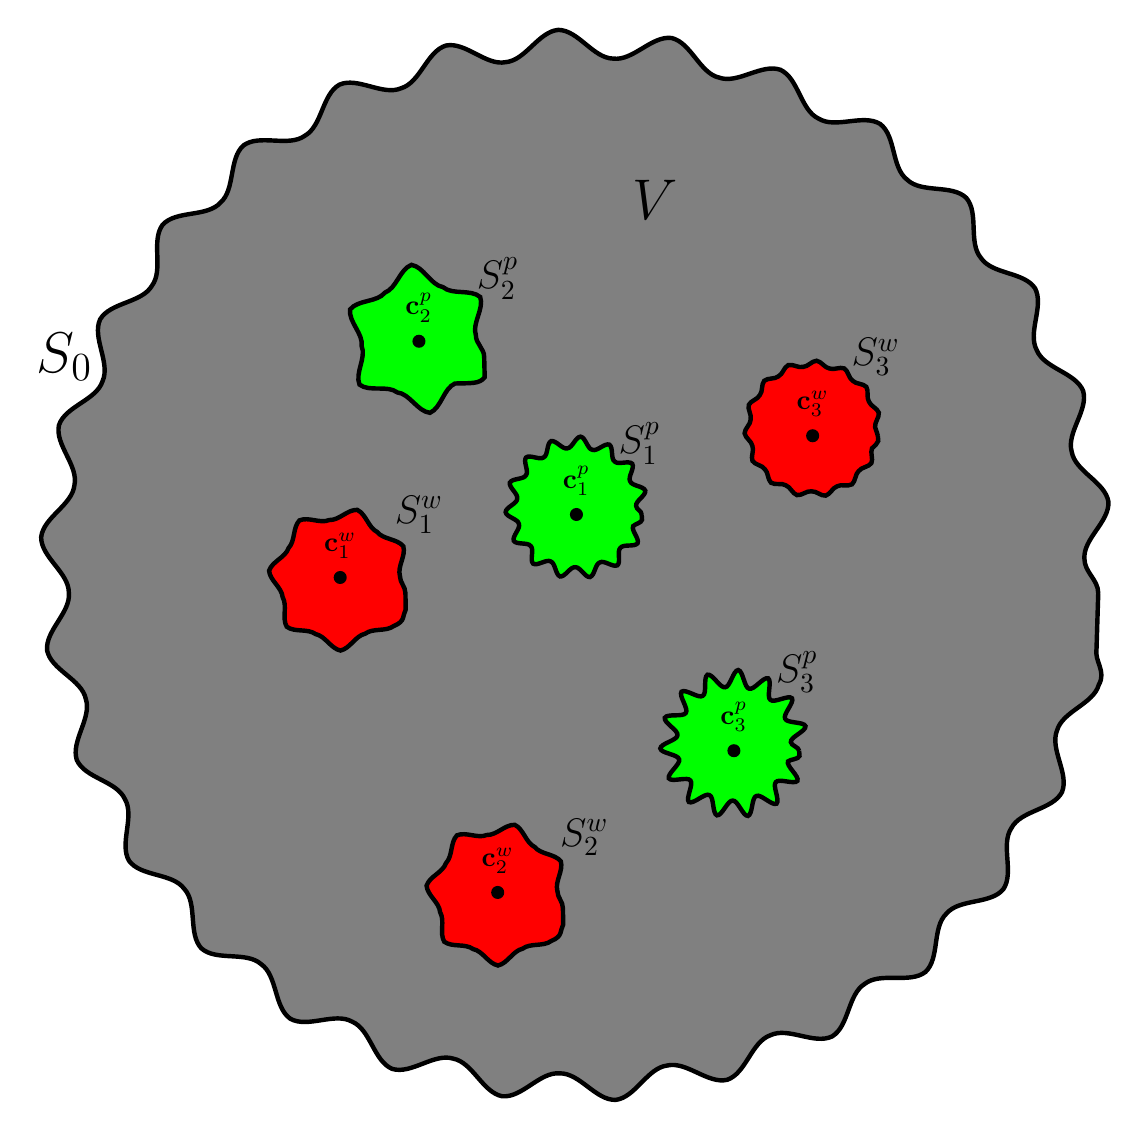
\begin{tikzpicture}[ultra thick]
		 \draw(0,0) node[circle,decorate, decoration={snake,amplitude=5pt,segment length=40pt},draw,scale=40,fill=gray] {};
	          \draw(0,1) node[circle,decorate, decoration={snake,amplitude=2pt,segment length=10pt},draw,scale=5,fill=green]{};
	          \draw(0,1) node[fill=black,circle,scale=0.5,label=above:{$\mathbf{c}^p_1$}]{};
	          \draw(0.8,1.9)node{\Large$S^p_1$};
	          \draw(-3,0) node[circle,decorate, decoration={snake,amplitude=2pt,segment length=20pt},draw,scale=5,fill=red]{};
	           \draw(-3,0.2) node[fill=black,circle,scale=0.5,label=above:{$\mathbf{c}^w_1$}]{};
	           \draw(-2,1)node{\Large$S^w_1$};
	          \draw(-2,3) node[circle,decorate, decoration={snake,amplitude=3pt,segment length=25.13 pt},draw,scale=5,fill=green]{};
	           \draw(-2,3.2) node[fill=black,circle,scale=0.5,label=above:{$\mathbf{c}^p_2$}]{};
	            \draw(-1,4)node{\Large$S^p_2$};
	          \draw(-1,-4) node[circle,decorate, decoration={snake,amplitude=2pt,segment length=20pt},draw,scale=5,fill=red]{};
	          \draw(-1,-3.8) node[fill=black,circle,scale=0.5,label=above:{$\mathbf{c}^w_2$}]{};
	           \draw(0.1,-3.1)node{\Large$S^w_2$};
	          \draw(2,-2) node[circle,decorate, decoration={snake,amplitude=3pt,segment length=10pt},draw,scale=5,fill=green]{};
	          \draw(2,-2) node[fill=black,circle,scale=0.5,label=above:{$\mathbf{c}^p_3$}]{};
	           \draw(2.8,-1)node{\Large$S^p_3$};
	          \draw(3,2) node[circle,decorate, decoration={snake,amplitude=1pt,segment length=10pt},draw,scale=5,fill=red]{};
	          \draw(3,2) node[fill=black,circle,scale=0.5,label=above:{$\mathbf{c}^w_3$}]{};
	           \draw(3.8,3)node{\Large$S^w_3$};
	          \draw(1,5)node{\huge$V$};
	           \draw(-6.5,3)node{\huge$S_0$};
	           
\end{tikzpicture}
\end{document}
